
%% bare_conf.tex
%% V1.3
%% 2007/01/11
%% by Michael Shell
%% See:
%% http://www.michaelshell.org/
%% for current contact information.
%%
%% This is a skeleton file demonstrating the use of IEEEtran.cls
%% (requires IEEEtran.cls version 1.7 or later) with an IEEE conference paper.
%%
%% Support sites:
%% http://www.michaelshell.org/tex/ieeetran/
%% http://www.ctan.org/tex-archive/macros/latex/contrib/IEEEtran/
%% and
%% http://www.ieee.org/

%%*************************************************************************
%% Legal Notice:
%% This code is offered as-is without any warranty either expressed or
%% implied; without even the implied warranty of MERCHANTABILITY or
%% FITNESS FOR A PARTICULAR PURPOSE! 
%% User assumes all risk.
%% In no event shall IEEE or any contributor to this code be liable for
%% any damages or losses, including, but not limited to, incidental,
%% consequential, or any other damages, resulting from the use or misuse
%% of any information contained here.
%%
%% All comments are the opinions of their respective authors and are not
%% necessarily endorsed by the IEEE.
%%
%% This work is distributed under the LaTeX Project Public License (LPPL)
%% ( http://www.latex-project.org/ ) version 1.3, and may be freely used,
%% distributed and modified. A copy of the LPPL, version 1.3, is included
%% in the base LaTeX documentation of all distributions of LaTeX released
%% 2003/12/01 or later.
%% Retain all contribution notices and credits.
%% ** Modified files should be clearly indicated as such, including  **
%% ** renaming them and changing author support contact information. **
%%
%% File list of work: IEEEtran.cls, IEEEtran_HOWTO.pdf, bare_adv.tex,
%%                    bare_conf.tex, bare_jrnl.tex, bare_jrnl_compsoc.tex
%%*************************************************************************
\documentclass[9pt]{sig-alternate}

%\usepackage[compact]{titlesec}
%\titlespacing{\section}{0pt}{*0}{*0}

%\usepackage{biblatex}
%\usepackage{amsmath}
%\usepackage{amssymb}
%\usepackage{times}
%\usepackage{hyperref}
%\usepackage{graphicx}
\usepackage{wrapfig}
\usepackage{listings}
\usepackage[usenames,dvipsnames]{xcolor}
%\usepackage{setspace}
\usepackage{python_syntax}
%\usepackage{bibentry}
\usepackage{todonotes}
\usepackage{url}
\usepackage{lineno}
%\usepackage{natbib}
%\usepackage{caption}
\usepackage[english]{babel} 
\def\UrlFont{\em} % Italicize all URLs.  
\lstset{
	basicstyle=\footnotesize\ttfamily,
	breaklines=true,
	language=Python,
	}
\newcommand{\verbx}[1]{\lstinline{#1}}
\newcommand{\bfhead}[1]{\noindent \textbf{#1:}}

\usepackage{alltt}
\renewcommand{\ttdefault}{txtt}

%\titlespacing{\subsection}{0pt}{*0}{*0}
%\titlespacing{\subsubsection}{0pt}{*0}{*0}

%%\usepackage{color}
%%\usepackage[usenames,dvipsnames,svgnames,table]{xcolor}
%%\definecolor{mauve}{rgb}{0.58,0,0.82}
%\definecolor{light-gray}{gray}{0.75}
%\usepackage{listings}
%\lstset{
%  language=Python,
%  showstringspaces=false,
%  formfeed=\newpage,
%  tabsize=4,
%  commentstyle=\itshape,
%  basicstyle=\ttfamily\scriptsize,
%  morekeywords={lambda, self, assert, as},
%  numbers=left,
%  numberstyle=\scriptsize\color{light-gray}\textsf,
%  xleftmargin=2em,
%  stringstyle=\color{mauve}
%}
%\lstdefinestyle{Bash}{
%    language={}, 
%    moredelim=**[is][\color{blue}\bf\ttfamily]{`}{`},
%}
%\lstdefinestyle{OpenCL}{
%	language=C++,
%	morekeywords={kernel, __kernel, global, __global, size_t, get_global_id, sin}
%}
%
%\usepackage{float}
%\floatstyle{ruled}
%\newfloat{codelisting}{tp}{lop}
%\floatname{codelisting}{Listing}

% *** GRAPHICS RELATED PACKAGES ***
%
% *** MATH PACKAGES ***
%
%\usepackage[cmex10]{amsmath}
% A popular package from the American Mathematical Society that provides
% many useful and powerful commands for dealing with mathematics. If using
% it, be sure to load this package with the cmex10 option to ensure that
% only type 1 fonts will utilized at all point sizes. Without this option,
% it is possible that some math symbols, particularly those within
% footnotes, will be rendered in bitmap form which will result in a
% document that can not be IEEE Xplore compliant!
%
% Also, note that the amsmath package sets \interdisplaylinepenalty to 10000
% thus preventing page breaks from occurring within multiline equations. Use:
%\interdisplaylinepenalty=2500
% after loading amsmath to restore such page breaks as IEEEtran.cls normally
% does. amsmath.sty is already installed on most LaTeX systems. The latest
% version and documentation can be obtained at:
% http://www.ctan.org/tex-archive/macros/latex/required/amslatex/math/

% *** SPECIALIZED LIST PACKAGES ***
%
%\usepackage{algorithmic}
% algorithmic.sty was written by Peter Williams and Rogerio Brito.
% This package provides an algorithmic environment fo describing algorithms.
% You can use the algorithmic environment in-text or within a figure
% environment to provide for a floating algorithm. Do NOT use the algorithm
% floating environment provided by algorithm.sty (by the same authors) or
% algorithm2e.sty (by Christophe Fiorio) as IEEE does not use dedicated
% algorithm float types and packages that provide these will not provide
% correct IEEE style captions. The latest version and documentation of
% algorithmic.sty can be obtained at:
% http://www.ctan.org/tex-archive/macros/latex/contrib/algorithms/
% There is also a support site at:
% http://algorithms.berlios.de/index.html
% Also of interest may be the (relatively newer and more customizable)
% algorithmicx.sty package by Szasz Janos:
% http://www.ctan.org/tex-archive/macros/latex/contrib/algorithmicx/

% *** ALIGNMENT PACKAGES ***
%
%\usepackage{array}
% Frank Mittelbach's and David Carlisle's array.sty patches and improves
% the standard LaTeX2e array and tabular environments to provide better
% appearance and additional user controls. As the default LaTeX2e table
% generation code is lacking to the point of almost being broken with
% respect to the quality of the end results, all users are strongly
% advised to use an enhanced (at the very least that provided by array.sty)
% set of table tools. array.sty is already installed on most systems. The
% latest version and documentation can be obtained at:
% http://www.ctan.org/tex-archive/macros/latex/required/tools/

%\usepackage{mdwmath}
%\usepackage{mdwtab}
% Also highly recommended is Mark Wooding's extremely powerful MDW tools,
% especially mdwmath.sty and mdwtab.sty which are used to format equations
% and tables, respectively. The MDWtools set is already installed on most
% LaTeX systems. The lastest version and documentation is available at:
% http://www.ctan.org/tex-archive/macros/latex/contrib/mdwtools/

% IEEEtran contains the IEEEeqnarray family of commands that can be used to
% generate multiline equations as well as matrices, tables, etc., of high
% quality.

%\usepackage{eqparbox}
% Also of notable interest is Scott Pakin's eqparbox package for creating
% (automatically sized) equal width boxes - aka "natural width parboxes".
% Available at:
% http://www.ctan.org/tex-archive/macros/latex/contrib/eqparbox/

% *** SUBFIGURE PACKAGES ***
%\usepackage[tight,footnotesize]{subfigure}
% subfigure.sty was written by Steven Douglas Cochran. This package makes it
% easy to put subfigures in your figures. e.g., "Figure 1a and 1b". For IEEE
% work, it is a good idea to load it with the tight package option to reduce
% the amount of white space around the subfigures. subfigure.sty is already
% installed on most LaTeX systems. The latest version and documentation can
% be obtained at:
% http://www.ctan.org/tex-archive/obsolete/macros/latex/contrib/subfigure/
% subfigure.sty has been superceeded by subfig.sty.

%\usepackage[caption=false]{caption}
%\usepackage[font=footnotesize]{subfig}
% subfig.sty, also written by Steven Douglas Cochran, is the modern
% replacement for subfigure.sty. However, subfig.sty requires and
% automatically loads Axel Sommerfeldt's caption.sty which will override
% IEEEtran.cls handling of captions and this will result in nonIEEE style
% figure/table captions. To prevent this problem, be sure and preload
% caption.sty with its "caption=false" package option. This is will preserve
% IEEEtran.cls handing of captions. Version 1.3 (2005/06/28) and later 
% (recommended due to many improvements over 1.2) of subfig.sty supports
% the caption=false option directly:
%\usepackage[caption=false,font=footnotesize]{subfig}
%
% The latest version and documentation can be obtained at:
% http://www.ctan.org/tex-archive/macros/latex/contrib/subfig/
% The latest version and documentation of caption.sty can be obtained at:
% http://www.ctan.org/tex-archive/macros/latex/contrib/caption/

% *** FLOAT PACKAGES ***
%
%\usepackage{fixltx2e}
% fixltx2e, the successor to the earlier fix2col.sty, was written by
% Frank Mittelbach and David Carlisle. This package corrects a few problems
% in the LaTeX2e kernel, the most notable of which is that in current
% LaTeX2e releases, the ordering of single and double column floats is not
% guaranteed to be preserved. Thus, an unpatched LaTeX2e can allow a
% single column figure to be placed prior to an earlier double column
% figure. The latest version and documentation can be found at:
% http://www.ctan.org/tex-archive/macros/latex/base/

%\usepackage{stfloats}
% stfloats.sty was written by Sigitas Tolusis. This package gives LaTeX2e
% the ability to do double column floats at the bottom of the page as well
% as the top. (e.g., "\begin{figure*}[!b]" is not normally possible in
% LaTeX2e). It also provides a command:
%\fnbelowfloat
% to enable the placement of footnotes below bottom floats (the standard
% LaTeX2e kernel puts them above bottom floats). This is an invasive package
% which rewrites many portions of the LaTeX2e float routines. It may not work
% with other packages that modify the LaTeX2e float routines. The latest
% version and documentation can be obtained at:
% http://www.ctan.org/tex-archive/macros/latex/contrib/sttools/
% Documentation is contained in the stfloats.sty comments as well as in the
% presfull.pdf file. Do not use the stfloats baselinefloat ability as IEEE
% does not allow \baselineskip to stretch. Authors submitting work to the
% IEEE should note that IEEE rarely uses double column equations and
% that authors should try to avoid such use. Do not be tempted to use the
% cuted.sty or midfloat.sty packages (also by Sigitas Tolusis) as IEEE does
% not format its papers in such ways.

% *** PDF, URL AND HYPERLINK PACKAGES ***
%
% url.sty was written by Donald Arseneau. It provides better support for
% handling and breaking URLs. url.sty is already installed on most LaTeX
% systems. The latest version can be obtained at:
% http://www.ctan.org/tex-archive/macros/latex/contrib/misc/
% Read the url.sty source comments for usage information. Basically,
% \url{my_url_here}.

%\usepackage{placeins}

% *** Do not adjust lengths that control margins, column widths, etc. ***
% *** Do not use packages that alter fonts (such as pslatex).         ***
% There should be no need to do such things with IEEEtran.cls V1.6 and later.
% (Unless specifically asked to do so by the journal or conference you plan
% to submit to, of course. )


% correct bad hyphenation here
\hyphenation{op-tical net-works semi-conduc-tor}

\usepackage{enumitem}
\setenumerate{noitemsep,topsep=2pt,parsep=0pt,partopsep=0pt}
\newcommand{\subparagraph}{}
\usepackage[compact]{titlesec}
\titlespacing{\section}{0pt}{*0.2}{*0}
%\titleformat{\section}
%  {\large\bfseries\uppercase}{\thesection}{1em}{}
\titlespacing{\subsection}{0pt}{*0}{*0}
\titlespacing{\subsubsection}{0pt}{*0}{*0}


\begin{document}
\conferenceinfo{ICSE}{'14, May 31 - June 7, 2014, Hyderabad, India}
\CopyrightYear{2014}
\crdata{978-1-4503-2768-8/14/05}
%
% paper title
% can use linebreaks \\ within to get better formatting as desired
\title{Collaborative Infrastructure for Test-Driven \\Scientific Model Validation}


% author names and affiliations
% use a multiple column layout for up to two different
% affiliations
\numberofauthors{2}
\author{\alignauthor
Cyrus Omar, Jonathan Aldrich\\\affaddr{Carnegie Mellon University, USA}\\
       {\{comar,aldrich\}@cs.cmu.edu}
       \alignauthor Richard C. Gerkin\\
       \affaddr{Arizona State University, USA}\\{rgerkin@asu.edu}
}

% conference papers do not typically use \thanks and this command
% is locked out in conference mode. If really needed, such as for
% the acknowledgment of grants, issue a \IEEEoverridecommandlockouts
% after \documentclass

% for over three affiliations, or if they all won't fit within the width
% of the page, use this alternative format:
% 
%\author{\IEEEauthorblockN{Michael Shell\IEEEauthorrefmark{1},
%Homer Simpson\IEEEauthorrefmark{2},
%James Kirk\IEEEauthorrefmark{3}, 
%Montgomery Scott\IEEEauthorrefmark{3} and
%Eldon Tyrell\IEEEauthorrefmark{4}}
%\IEEEauthorblockA{\IEEEauthorrefmark{1}School of Electrical and Computer Engineering\\
%Georgia Institute of Technology,
%Atlanta, Georgia 30332--0250\\ Email: see http://www.michaelshell.org/contact.html}
%\IEEEauthorblockA{\IEEEauthorrefmark{2}Twentieth Century Fox, Springfield, USA\\
%Email: homer@thesimpsons.com}
%\IEEEauthorblockA{\IEEEauthorrefmark{3}Starfleet Academy, San Francisco, California 96678-2391\\
%Telephone: (800) 555--1212, Fax: (888) 555--1212}
%\IEEEauthorblockA{\IEEEauthorrefmark{4}Tyrell Inc., 123 Replicant Street, Los Angeles, California 90210--4321}}




% use for special paper notices
%\IEEEspecialpapernotice{(Invited Paper)}




% make the title area
\maketitle

\begin{abstract}
One of the pillars of the modern scientific method is \emph{model validation}: comparing a scientific model's predictions against empirical observations. Today, a scientist demonstrates the validity of a model by making an argument in a paper and submitting it for peer review, a process comparable to \emph{code review} in software engineering. While human review helps to ensure that contributions meet high-level goals, software engineers typically supplement it with \emph{unit testing} to get a more complete picture of the status of a project.%, particularly one involving many contributors.

We argue that a similar test-driven methodology would be valuable to scientific communities as they seek to  validate increasingly complex models against growing repositories of empirical data. Scientific communities differ from software communities in several key ways, however. In this paper, we introduce \emph{SciUnit}, a framework for test-driven scientific model validation, and outline how, supported by new and existing collaborative infrastructure, it could integrate into the modern scientific process.
\end{abstract}
\category{D.2.5}{Software Engineering}{Testing and Debugging}%[complexity measures, performance measures]
\terms{Documentation, Measurement, Standardization}
\keywords{unit testing, model validation, cyberinfrastructure}

%\begin{IEEEkeywords}
%unit testing, validation, computer-supported collaborative work
%\end{IEEEkeywords}


% For peer review papers, you can put extra information on the cover
% page as needed:
% \ifCLASSOPTIONpeerreview
% \begin{center} \bfseries EDICS Category: 3-BBND \end{center}
% \fi
%
% For peerreview papers, this IEEEtran command inserts a page break and
% creates the second title. It will be ignored for other modes.
%\IEEEpeerreviewmaketitle
\titleformat{\section}
 {\secfnt}{\thesection.}{1em}{\secfnt\MakeUppercase}
 \vspace{10pt}
\section{Introduction}
\begin{figure*}[t]
\vspace{-30px}
\centering
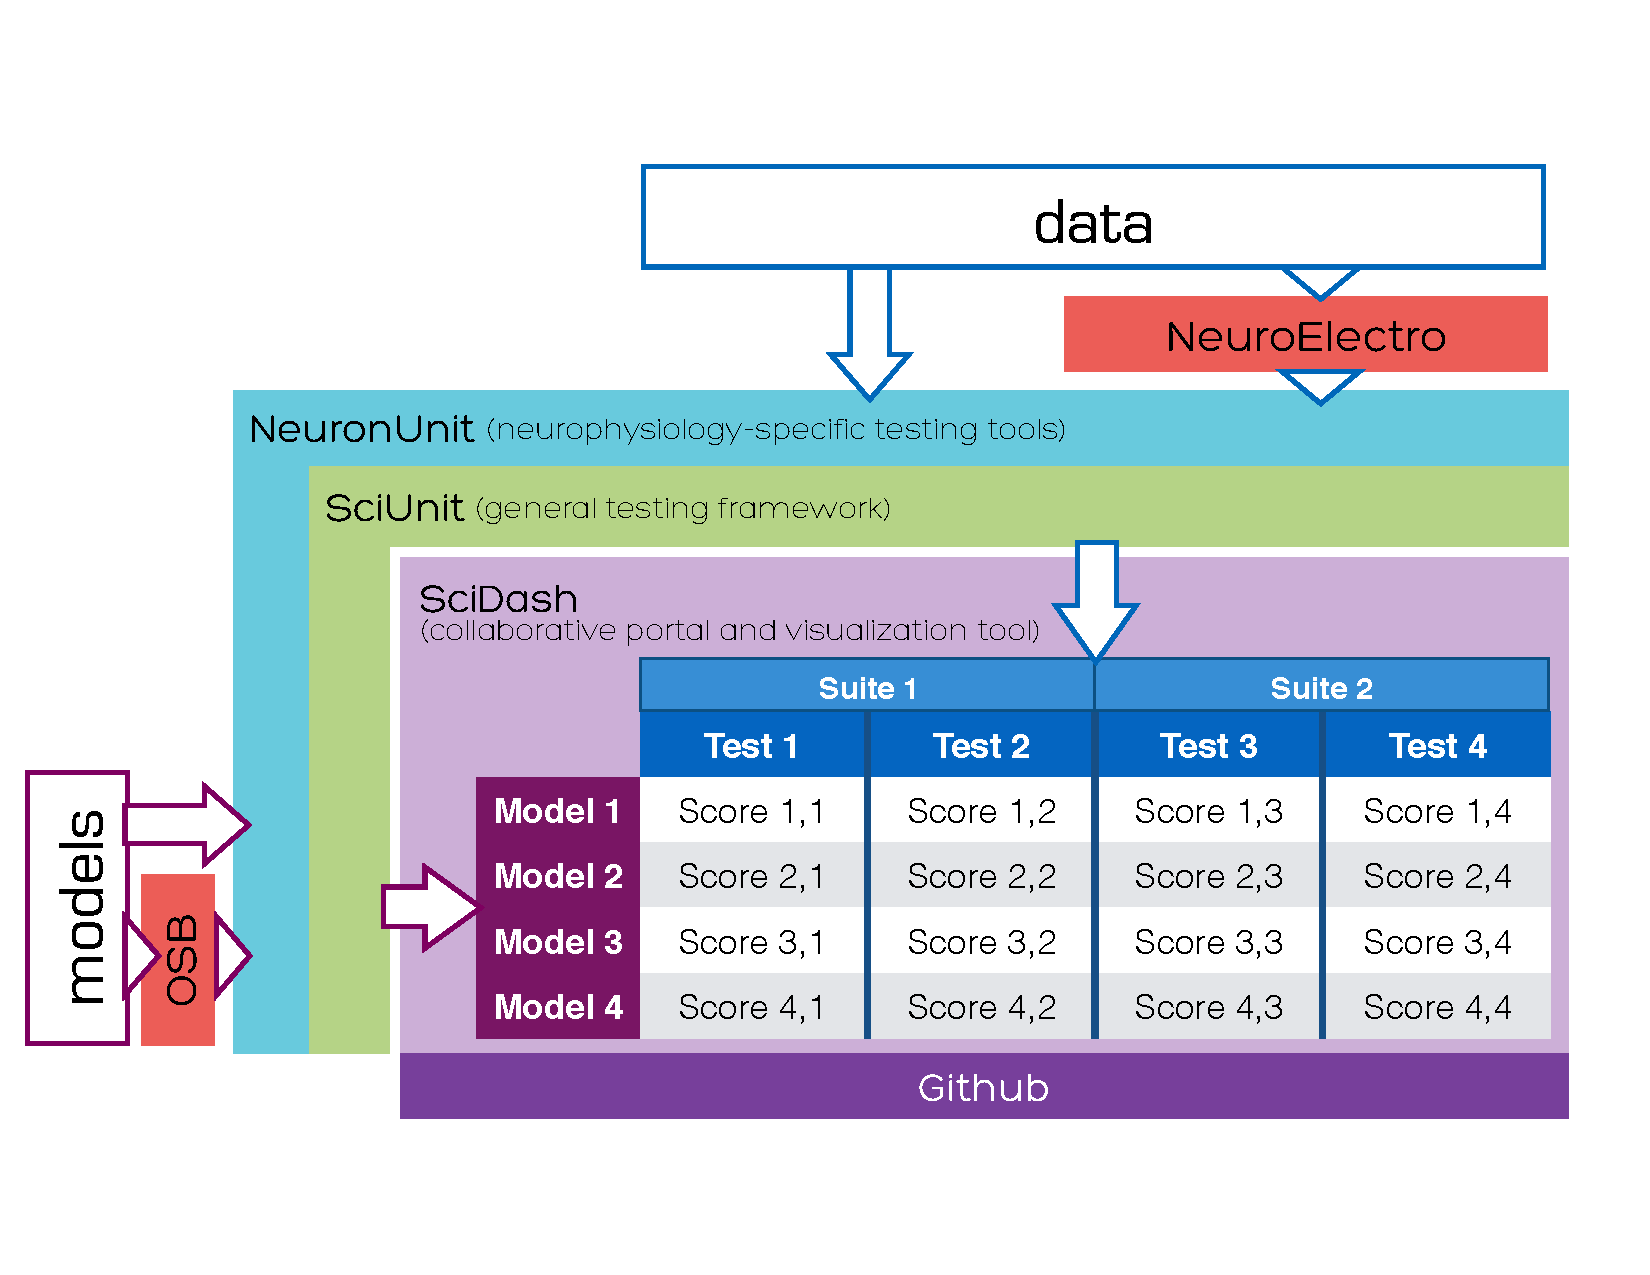
\includegraphics[scale=0.45]{diagram1.pdf}
\vspace{-50px}
\caption{\small Tests are derived from data and models are derived from scientific theories, either directly or through existing data and model repositories. The score table (center) summarizes the performance of a collection of models against a suite of tests. Tests and models are initialized, executed and visualized using \texttt{sciunit} in an IPython notebook stored inside a \emph{suite repository} (e.g. \texttt{saturnsuite}) hosted on a social coding website (e.g. Github). SciDash  discovers and organizes  suite repositories and provides utilities for viewing them online without needing to create a local copy. Logic common across research areas is also collaboratively developed (e.g. \texttt{cosmounit}).}  
\label{fig:sciunit_overview}
\vspace{-10pt}
\end{figure*}


Scientific theories are increasingly being organized around \emph{quantitative models}:  formal systems capable of generating predictions about observable quantities. A model can be  characterized by its \textit{scope}: the set of observable quantities that it attempts to predict, and by its \textit{validity}: the extent to which its predictions agree with experimental observations of these quantities. 

Today, quantitative models are validated by \emph{peer review}. For a model to be accepted by a scientific community, its advocates must submit a paper that describes how it works and provides evidence that it makes more accurate predictions than previous models (or that it makes a desirable tradeoff  between accuracy and complexity) \cite{box1987empirical}. Other members of the relevant community are then tasked with ensuring that validity was measured correctly and that all relevant data and competing models were adequately considered, drawing on knowledge of statistical methods and the prior literature. Publishing is a primary motivator for most scientists \cite{howison2011scientific}.

Quantitative scientific modeling shares much in common with software development. Indeed, quantitative models are increasingly being implemented in software and in some cases, the software \emph{is} the model (e.g. complex simulations). The peer review process for papers is similar in many ways to the \emph{code review} process used in many development teams, where team members look for mistakes, enforce style and architectural guidelines and check that the code is \emph{valid} (i.e. that it achieves its intended goal) before permitting it to be committed to the primary source code repository. 


Code review can be quite effective \cite{codereview}, but this requires that developers  expend considerable effort \cite{kemerer2009impact}. 
%Code review is also most effective for resolving  issues related to software architecture. 
Most large development teams thus supplement code reviews with more {automated} approaches to verification and validation, the most widely-used  of which is \emph{unit testing} \cite{beck2003}. In brief, unit tests are functions that check that the behavior of a single component satisfies a single functional  criterion. 
%A suite of such tests can be considered a partial specification of the program or component under development.  
A suite of such tests complements code review by making it easier to answer questions like these:
\begin{enumerate}
\item What functionality is a component expected to have?
\item What functionality has been adequately implemented? What remains to be done?
%\item How much progress does an individual code contribution make? 
\item Does a candidate code contribution cause \emph{regressions} in other parts of a program?
\end{enumerate}
Scientists ask analagous questions:
\begin{enumerate}
\item What is a model's scope and how is validity measured?
\item Which observations are already explained by existing models? What are the best models of a particular quantity?  What data has yet to be explained?
%\item How much better is a new model than the state of the art? What are the open problems in my field?
\item What affect do new observations have on the validity of previously published models? Can new models explain previously published data?
\end{enumerate}
But while software engineers can rely on a program's test suite, scientists today must extract this information from a body of scientific papers. This is increasingly difficult. Each paper is narrowly focused, often considering just one model or dataset, and is frozen in time, so it does not consider the latest models, data or statistical methods. Discovering, precisely characterizing and comparing models to determine the state of the art and find open modeling problems can require an encyclopedic knowledge of the literature, as can finding all data relevant to a model. Senior scientists often attempt to fill these needs by publishing review papers, but in many areas, the number of publications generated every year can be overwhelming \cite{jinha_article_2010}, and comprehensive reviews of a particular area are published infrequently. Statisticians often complain that scientists are not following best practices and that community standards evolve too slowly because a canonical paper or popular review relied on outdated methods. Furthermore, if the literature simply doesn't address an important question of validity (e.g. if space was limited), a researcher might need to reimplement an existing model from scratch to attempt to address it. 

One might compare this to a large software development team answering the questions listed above based largely on carefully reviewed, but rarely updated,  API documentation and annual high-level project summaries.
While certainly a caricature, this motivates our suggestion that the scientific process could be improved by the adoption of test-driven methodologies alongside traditional peer review. However, the scientific community presents several unique challenges:
\begin{enumerate}
\item Unit tests are typically pass/fail, while goodness-of-fit between a model and data is typically measured by a continuous metric. 
\item Unit tests often test a \emph{particular} component, whereas a \emph{validation testing} system must be able to handle and compare many models with the same scope. %They are sometimes reluctant to share certain details of their implementations \cite{badscientists}.
%\item Experimental data can itself be erroneous, noisy or inconsistent with other available data.
\item Scientists use a variety of programming languages.
\item Scientists often only loosely coordinate their efforts.
\item Different communities, groups and individuals prefer different goodness-of-fit metrics and focus on different sets of observable quantities. In contrast, there is more pressure to agree upon requirements and priorities in a typical software development project.
\item Professional software developers are typically trained in testing practices and the use of collaborative tools, while scientists more rarely have such experience \cite{oai:open.ac.uk.OAI2:17673}. %Thus, the framework must be as simple as possible.
\end{enumerate}

To begin to address these challenges, we will introduce a lightweight and flexible validation testing and framework called \textit{SciUnit} in Sec. 2. Many of these challenges have to do with coordination between scientists. To begin to address this, we then describe a community workflow based on widely-adopted social coding tools (here, Github) and a lightweight community portal called \textit{SciDash}, in Sec. \ref{scidash}. The overall goal of this work is to help scientists generate tables like the one central to Figure 1, where the relative validity of a set of models having a common scope can be determined by examining scores produced by a suite of validation tests constructed from experimental data. 
We discuss adoption strategies and conclude in Sec. \ref{discussion} with directions for future research into scientific model validation practices.
%Anecdotally, one of the greatest fears of new scientists is that a problem that they are working on has already been solved and published. 


%This suggests that tools that help researchers answer questions like these could help readers and reviewers develop a more comprehensive understanding of the state-of-the-art and improve the quality of the research being published as a result: to renewed calls for tools that help researchers . 

%These questions are particularly relevant for young scientists and  scientists aiming to enter a new research area to answer.

%understanding of the state-of-the-art from publications containing only a few pieces of data, and then only that data available at the time of publication. 

%These demonstrations also quickly go out of date. Finally, there is no easy way to summarize and compare the claims being made in modeling papers in order to synthesize an understanding of a research area as a whole. 
%A strength of publications are their focused descriptions of new data and models. 
%A weakness, however, is that evaluating the scope and validity of models against known data is intractable using a body of publications alone.

%publications would be analagous to user manuals, rather than rigorous justifications that a program meets a specific specification. Unit tests serve this purpose for software, so we argue that the validation of neuroscience models by means of executable tests would be useful to scientists as a supplement the publication system.
% In addition to this open testing toolkit we also provide a library of tests for models of spiking single neurons.  

% Section 2.
\section{Validation Testing with {SciUnit}}

%Simple executable \emph{validation tests} that compute agreement between a model prediction and an experimental observation.  
As a motivating example, we will begin by considering a community of early cosmologists recording and attempting to model observations of the planets visible in the sky, such as their position, velocity, orbital eccentricity and so on. One simple validation test might ask a model to predict planetary position on night $n+1$ given observations of its position on $n$ previous nights. Figure 2 shows how to implement a test, using  SciUnit, that captures this logic.

Before explaining the details of this example, we point out that SciUnit is implemented in Python. Python is one of the most widely used languages in science today \cite{sanner1999python}, and is increasingly regarded as the \textit{de facto} language of open source scientific computing. It is easy to read and has a simple object system that we use to specify the interface between tests and models (challenge 2, see below). It supports calling into other popular languages, including R, MATLAB, C and Java, often more cleanly than they support calling into Python (challenge 3). The IPython notebook is a powerful web-based ``read-eval-visualize loop'' that we will use to support interactive table visualization, and it also permits using other languages on a per-cell basis \cite{perez2007ipython}. Together, this makes writing wrappers around tests and models written in other languages relatively simple. We anticipate making it nearly automatic as future work.
\begin{figure}[t]
\small
%class PositionTest(sciunit.Test):
%    """Tests a planetary position model based on positions observed on night n given the positions in the n-1 previous nights.
%    Metric: Standard p-value.
%    Parameters: 
%      obs_histories : list[list[position]]
%      obs_positions: list[position]"""
%	def __init__(self, obs_histories, obs_positions):
%		self.obs_histories = obs_histories
%		self.obs_positions = obs_positions
%
%	required_capabilities = [PredictsPlanetaryPosition]
%
%	def _judge(self, model):
%		predictions = []
%		for obs_history in self.obs_histories:
%			predictions.append(model.predict_next_pos(obs_history))
%		p = pooled_p_val(predictions, self.obs_positions)
%		return sciunit.PValue(p, related_data={
%			'obs_histories': obs_histories,
%			'obs_positions': obs_positions,
%			'predictions': predictions
%		})
\begin{python}
class PositionTest(sciunit.Test):
  """Tests a planetary position model based on positions observed on night n given the positions in the n-1 previous nights.
  Observation: {
    'histories':list[list[Position]], 
    'positions':list[Position]]
  }"""
  required_capabilities = [PredictsPlanetaryPosition]
  def generate_prediction(self, model):
    return [model.predict_next_pos(obs_history)
      for obs_history 
      in self.observation['histories']]

  def compute_score(self, observation, prediction):
    obs_positions = observation['positions']
    return pooled_p_val([abs_distance(obs, pred)
      for (obs, pred) 
      in zip(obs_positions, prediction)])
\end{python}
\vspace{-12px}
\caption{\small An example test class in \texttt{cosmounit}.}
\label{fig:rate_test}
\vspace{-15px}
\end{figure}

A {SciUnit} validation test is an {instance} of a Python class inheriting from  \verbx{sciunit.Test} (line 1). 
Every test takes one required constructor argument (inherited from the base class): the observation(s) against which the test will validate models.
In our example, this is a dictionary, documented per Python conventions on lines 2-6. 
%For convenience, we also make use of functions provided by the popular NumPy\cite{numpy_url} and SciPy\cite{scipy_url} libraries, although these are not required by \textit{SciUnit}.  
To create a \emph{particular} position test, we instantiate this class with particular observations. 
For example, the subset of cosmologists interested specifically in Saturn might instantiate a test by randomly chunking observations made about Saturn's nightly position over time as follows:
\vspace{-3px}
\begin{python}
  h, p = randomly_chunk(obsvd_saturn_positions)
  saturn_position_test = PositionTest(
    {'histories': h, 'positions': p})
\end{python}
\vspace{-5px}
The class \verb|PositionTest| defines logic that is not specific to any particular planet, so it is contained in a repository shared by all cosmologists called \verbx{cosmounit}. The particular test above would be constructed in a separate repository focused specifically on Saturn called \verbx{saturnsuite}. Both would be collaboratively developed by these (overlapping) research communities in source code repositories on Github.

Classes that implement the \verbx{sciunit.Test} interface must specify two methods: a method for extracting a prediction from a model, and a method for producing a score from that prediction. Predictions are extracted by a separate method to make it easier for statisticians to write new tests for which only the goodness-of-fit metric differs, not the method by which the prediction is extracted (challenge 5).

The \verbx{generate_prediction} method (lines 8-11) is passed a \emph{model} as input and must extract a \emph{prediction}. A model is an instance of a class inheriting from \verbx{sciunit.Model} and a prediction can be any Python data structure. To specify the interface between the test and the model, the test class specifies a list of \verbx{required_capabilities} (line 7). 
A capability specifies the methods that a test may need to invoke on the model to extract a prediction, and is analogous to an \emph{interface} in a language like Java. 
In Python, capabilities are written as classes with unimplemented members, shown in Figure \ref{fig:capability}. 
Classes defining capabilities are tagged as such by inheriting from \verbx{sciunit.Capability}. The test in Figure \ref{fig:rate_test} repeatedly uses this capability on lines 9-11 to return a list of predicted positions for each observed history (using a list comprehension for brevity).  A planet's position is represented using a standard celestial coordinate system specified within \verbx{cosmounit} by the class \verbx{Position}. 

A model class implements a capability by inheriting from it and implementing the required methods (Figure \ref{fig:capability}).  The scope of a model class is identified by the capabilities it has. A particular model is an instance of such a class: 
\vspace{-3px}
\begin{python}
lin_saturn_model = LinearPlanetModel()
\end{python}
\vspace{-5px}

Once a prediction has been extracted from a model, the test class must compute a \emph{score}. The framework invokes the \verbx{compute_score} method with the observation provided upon test instantiation and the prediction just generated. On lines 13-17 of Fig. \ref{fig:rate_test}, the test class constructs a list of distances between the observed and predicted positions, then determines a pooled $p$-value to determine the goodness-of-fit (the details are omitted for concision). A $p$-value is represented as an instance of \verbx{sciunit.PValue}, a subclass of \texttt{sciunit.Score} that has been included with {SciUnit} due to its wide use across science. %In addition to the $p$-value itself, the returned score object also contains metadata, accessible via the \verbx{related_data} attribute, for  scientists who may wish to examine the result in more detail later. This includes the observation, prediction, and a reference to the model and test. 
\begin{figure}
\small
\begin{python}
class PredictsPlanetaryPosition(sciunit.Capability):
  def predict_next_pos(self, history): 
    """Takes a list of previous Positions and produces the next Position."""
    raise NotImplementedError()

class LinearPlanetModel(sciunit.Model, 
    PredictsPlanetaryPosition):
  def predict_next_pos(self, history):
    return linear_prediction(history)
\end{python}
\vspace{-12px}
\caption{\small An example capability and a model class that implements it in \verbx{cosmounit}.}
\label{fig:capability}
\vspace{-10px}
\end{figure}

This illustrates a key difference between unit testing, which would simply produce a boolean result, and our conception of scientific validation testing (challenge 1). A score class must induce an ordering, so that a table like that shown in Figure 1 can be sorted along its columns. A score class can also specify a normalization scheme so the cells of the table can be color-coded.  %It also makes it easier to cache predictions generated by large-scale models so that they can be used by multiple tests. 

The \verbx{judge} method of a test can be invoked to compute a score for a single model: 
\vspace{-4px}
\begin{python}
score = saturn_position_test.judge(lin_saturn_model)
\end{python}
\vspace{-5px}
This method first checks that the model implements all required capabilities, then calls the \verbx{generate_prediction} method, then passes the prediction to the \verbx{compute_score} method. A reference to the test,   model, observation, prediction and other related data the test provides (none here) are added as attributes of the score before it is returned.

To produce a comprehensive test suite, the contributors to \verbx{saturnsuite} would instantiate a number of other tests and then create an instance of the \verbx{TestSuite} class:
\begin{python}
saturn_motion_suite = sciunit.TestSuite([
  saturn_position_test, saturn_velocity_test, ...])
\end{python}
They would also instantiate a number of models. A test suite can be used to judge multiple models at once, if they satisfy the union of the capabilities required by the constituent tests (challenge 2). The result is a \emph{score matrix}:
\begin{python}
sm_matrix = saturn_motion_suite.judge([
  lin_saturn_model, ptolemy_model, kepler_model, ...])
\end{python}

If constructed inside an IPython notebook, a score matrix can then be visualized as an interactive table, much like the one shown in Figure \ref{fig:sciunit_overview}. Scientists can sort by column and click on tests, models and scores to get more information on each, including documentation, authorship information, related papers and other related data extracted from the underlying classes (details omitted for concision).

%They then defined a combined metric favoring models that broadly succeeded at meeting these criteria, to produce an overall ranking. 
%Such combined criteria are simply validation tests that invoke other tests to produce a result.
 
%In many cases, models require no modifications to take the new tests because the same type of model output is being requested.
%We discuss visualization of results in Secs. \ref{sec:scidash_activities} and \ref{sec:scidash_visualization}.

%\begin{figure}
%\begin{python}
%class TrainSpikeCountFromCurrent(sciunit.Capability):
%  def train_with_currents(self, currents, counts):
%    """Takes a list of numpy arrays containing current stimulus (in nA) and
%    observed spike counts. Model parameters should be adjusted based on this
%    training data."""
%    raise NotImplementedError("Model does not implement capability.")
%\end{python}
%\caption{Another capability specifying a training protocol (not used by the test in Figure \ref{fig:rate_test}).}
%\label{fig:training}
%\vspace{-15px}
%\end{figure}

%\subsection{Models}
%Capabilities are \emph{implemented} by models. In \textit{SciUnit}, models are instances of Python classes that inherit from \verbx{sciunit.Model}. Like tests, the class itself represents a family of models, parameterized by the arguments of the constructor. A particular model is an instance of such a class.
%
%Figure \ref{fig:simple_model} shows how to write a simple {family} of models, \verbx{LinearModel}, that implement the capability in Fig. \ref{fig:capability} as well as another capability shown in Fig. \ref{fig:training}, which we will discuss below. 
%Models in this family generate a spike count by applying a linear transformation to the mean of the provided input current. The family is parameterized by the scale factor and the offset of the transformation, both scalars. 
%To create a \emph{particular} linear model, a modeler can provide particular parameter values, just as with test families:
%\begin{python}
%CA1_linear_model_heuristic = LinearModel(3.0, 1.0)
%\end{python}
%Here, the parameters to the model were picked by the modeler heuristically, or based on externally-available knowledge. 
%An alternative test design would add a training phase where these parameters were fit to data using the capability shown in Fig. \ref{fig:training}. 
%This test could thus only be used for those models for which parameters can be adjusted without human involvement. 
%Whether to build a training phase into the test protocol is a choice left to each test development community. 
%
%Fig. \ref{fig:rate_test} does not include a training phase. 
%If training data is externally available, models that nevertheless do implement a training capability (like \verb|LinearModel|) can simply be trained explicitly by calling the capability method just like any other Python method:
%\begin{python}
%CA1_linear_model_fit = LinearModel()
%CA1_linear_model_fit.train_with_currents(CA1_training_in, CA1_training_out)
%\end{python}
%\begin{figure}
%\begin{python}
%class LinearModel(sciunit.Model, SpikeCountFromCurrent, 
%    TrainSpikeCountFromCurrent):
%  def __init__(self, scale=None, offset=None): 
%    self.scale, self.offset = scale, offset
%    
%  def spike_count_from_current(self, input):
%    return int(self.scale*numpy.mean(input) + self.offset)
%
%  def train_with_currents(self, currents, counts):
%    means = [numpy.mean(c) for c in currents]
%    [self.offset, self.scale] = numpy.polyfit(means, counts, deg=1)    
%\end{python}
%\caption{A model that returns a spike count by applying a linear transformation to the mean input current. The parameters can be provided manually or learned from data provided by a test or user (see text).}
%\label{fig:simple_model}
%\vspace{-15px}
%\end{figure}
%
\section{Collaborative Workflow}\label{scidash}

Social coding tools like Github allow each scientist to work on their own fork of a repository like \verbx{saturnunit} where they can examine the consequences of their own contributions on  the tests and models that have previously been developed. For example, an experimentalist who has gathered new data can instantiate a new test or refine an existing one  with more accurate observations. As long as the interface between the test and the model remains the same, the scores for prior models can be recomputed entirely automatically, requiring no coordination with model developers (challenge 4). When a modeler develops a new model, she can   validate it against all the tests it is capable of taking. If a statistician develops a better goodness-of-fit metric, she too can use existing capabilities and indeed inherit prediction extraction logic directly, as discussed above. If a scientist is not interested in certain tests, she can locally remove them to recalibrate her view of the relative merits of different models (challenge 5). 

If the changes to the repository appear to represent a contribution, these scientists might submit a \emph{pull request} to the central repository (either separately or together with the submission of a conventional paper). Anonymous reviewers tasked by the ``editors'' of the repository would then subject the pull request to appropriate peer review before committing it to the ``permanent record''. A model that performs well across tests in a collaboratively developed suite could more objectively claim (e.g. to reviewers) to be a coherent, valid model of, for example, Saturn's motion. 


%Because new models, tests and data are being added by a variety of people, there needs to be a collaborative workflow in place. As we have outlined above, the basic mechanisms have already been put in place by software developers. 

To help scientists discover and coordinate development of these repositories, we are developing a collaborative portal called \textit{SciDash} (\url{http://scidash.org/}). It is essentially a wiki pointing scientists to the repositories designated as ``primary'' by early adopters in their research areas (who may serve as \emph{de facto} initial editors as well). SciDash also supports loading IPython notebooks containing score tables stored in these repositories into the browser, avoiding the need to clone the repository locally. To modify the suite (e.g. to add the model a scientist is developing to it), a scientist can simply fork the repository by clicking a button at the top of this view. We are exploring ways of loading forks directly into a cloud-based IPython notebook system, so that the complexities of Git, Python setup and package management can be left behind the scenes (challenge 6). SciDash lists public forks of repositories that it is indexing to help scientists get a better sense of who is working on the problems they are interested in and what partial results are publicly available, fostering collaboration.

As with many pieces of cyberinfrastructure, early adopters may benefit less than late adopters due to network effects. To incentivize adoption, we look to an increasingly common scientific practice: modeling competitions. Many research communities use these to periodically determine the state of the art, resulting in a form of review paper (e.g. \cite{jolivet_quantitative_2008}). Funding sources often include small monetary incentives.
%For example, the quantitative single neuron modeling competition operated over the course of two years  \cite{qsnmc}. 
   SciDash could be used to run these kinds of competitions on a continuous basis atop less \textit{ad hoc} infrastructure (and thus require less effort and central planning from organizers) and we are actively recruiting organizers for such competitions.

%More directly: we anticipate common testing logic (e.g. \verbx{PositionTest}), modeling logic and capabilities being collaboratively developed by larger communities in less specialized repositories like \verbx{cosmounit}. Individuals and small groups will then parameterize these tests and models with data they have gathered, as well as data known from the literature and data contained in existing data repositories to create test suites in repositories like \verbx{saturnsuite}. The interface between data collection software and existing data representation standards and tests will be mediated by bridge logic also contained in repositories like \verbx{cosmounit}.  % This workflow is meant to evoke the \emph{test-driven development} methodology that is often used in software projects. 
%
%Statisticians wishing to promote new validation metrics can simply for a $X$\verbx{unit} repository and implement new test logic. By reusing the same interfaces as previous tests used, these new metrics can immediately be used to validate or invalidate a large body of existing models, providing valuable data for use in convincing the community to adopt these into the mainstream repositories. Similarly, investigators who wish to de-emphasize or emphasize different quantities can fork $X$\verbx{suite} repository and add or remove tests.

\vspace{5px}
\section{Discussion \& Future Directions}\label{discussion}
Instead of attempting to use an existing general-purpose testing framework (e.g. JUnit or PyUnit), we have designed what is essentially a domain-specific language that captures the scientific model validation process in more familiar terms (in view of challenge 6).% SciUnit can be used by individual scientists to organize their workflows using IPython notebooks \cite{perez2007ipython} and also within a loosely collaborative workflow, mediated by a social coding tool like Github and a simple portal, SciDash.

%Academic peer review and code review are similar, but software developers typically supplement human review with test-driven methodologies. Such methodologies may benefit scientific communities as well, but several unique  constraints make reusing existing testing frameworks and processes difficult. We describe a core testing framework that addresses these issues  by using an existing, widely-adopted language and designing a flexible, simple framework that captures the domain-specific structure of scientific model validation. We then describe, by example, how the various components can be organized into software repositories and collaboratively maintained using social coding tools to support existing scientific practices. We end by outlining a collaboratively filtered portal that sits atop these tools and facilitates exploratory analyses and repository discovery. 

While we discuss a simple example based on planetary movement here, we have applied this framework to more realistic problems in neurobiology in collaboration with the developers of two large-scale informatics projects, OpenSourceBrain and NeuroElectro, which serve as a source of models and data, respectively. Our tools serve, in essence, as a bridge between these resources. The tools we describe could also be used for a variety of other scientific disciplines, including within software engineering to validate predictive models of, for example, project duration or code reuse.

This work identifies new research directions in software engineering by developing connections between test-driven development \cite{beck2003} and the scientific model validation process, which has not been as extensively studied. Characterizing how scientists today attempt to answer the questions given in the introduction, evaluating how well sociotechnical solutions like the ones we propose here could improve their ability to do so, and studying adoption barriers are likely to be fruitful avenues for future empirical research, and lead to a better understanding of both programmers and scientists. 

The core SciUnit framework has been fully developed and is available at http://sciunit.scidash.org/. SciDash is under active development as of this writing.
\vspace{2px}
 %In particular, we consider modeling competitions in science as a form of test-driven validation. For example, the quantitative single neuron modeling competition (QSNMC) \cite{jolivet_quantitative_2008} investigates the complexity-accuracy tradeoff among reduced models of excitable membranes, and 
%examples from other subfields of biology abound (e.g. \url{http://www.the-dream-project.org}).  These competitions typically use \emph{ad hoc} infrastructure. A common framework could be used to make designing and continuously operating such contests more feasible. In related work that 

%Modeling competitions in neuroscience, for example, are typically organized around a collection of simple validation criteria, implemented as executable tests. 
%These competitions continue to drive important advances and improve scientists' understanding of the relative merits of different models. 
% \begin{figure}%{r}{0.6\textwidth}
% %\vspace{-38px}
% \includegraphics[scale=0.75]{sciunit_overview.pdf}
% \caption{Proposal overview. 
% \small{i) The \textit{SciUnit} framework can generate discipline-specific libraries for tests generation and model interfacing.  
% \textit{NeuronUnit} is proposed and described here.  Experimental data guides test development; model generation informs and is informed by these \textit{SciUnit} libraries.  
% Each \text{SciUnit} test suite repository on GitHub is indexed by the \textit{SciDash} web application.  
% Test suites for OSB and QSNMC (described in the text) are being built. 
% \textit{SciDash} automatically runs the test collections in each suite and publicly displays the results.}}
% %\vspace{-10px}
% \label{fig:sciunit_overview}
% \end{figure}
% \leavevmode
% \vspace{-0px}

%Each of these examples has leveraged \emph{ad hoc} infrastructure to support test generation. 
%While the specific criteria used to evaluate models varies widely between disciplines in neuroscience, the underlying test-driven methodology has many common features that could be implemented once. 
%Recognizing this, we developed a discipline-agnostic framework for developing scientific validation test suites called \textit{SciUnit} (\url{http://www.sciunit.org}). 

\section{ACKNOWLEDGEMENTS}
\vspace{-1px}
We thank Sharon Crook, Shreejoy Tripathy and Padraig Gleeson for their many helpful discussions, and anonymous referees and friends for their careful readings.  
RG was supported in part by NIMH grant R01MH081905. CO and JA were supported in part by NSF grant 1116907. 
The content is solely the responsibility of the authors and does not necessarily represent the official views of the NIH or NSF.
\vspace{2px}
% conference papers do not normally have an appendix


% use section* for acknowledgement
% trigger a \newpage just before the given reference
% number - used to balance the columns on the last page
% adjust value as needed - may need to be readjusted if
% the document is modified later
%\IEEEtriggeratref{8}
% The "triggered" command can be changed if desired:
%\IEEEtriggercmd{\enlargethispage{-5in}}

% references section

% can use a bibliography generated by BibTeX as a .bbl file
% BibTeX documentation can be easily obtained at:
% http://www.ctan.org/tex-archive/biblio/bibtex/contrib/doc/
% The IEEEtran BibTeX style support page is at:
% http://www.michaelshell.org/tex/ieeetran/bibtex/
%\bibliographystyle{IEEEtran}
% argument is your BibTeX string definitions and bibliography database(s)
%\bibliography{IEEEabrv,../bib/paper}
%
% <OR> manually copy in the resultant .bbl file
% set second argument of \begin to the number of references
% (used to reserve space for the reference number labels box)
%\renewcommand\bibsection{\subsection{\refname}}
\bibliographystyle{abbrv}
\bibliography{../research,references,references_crook,urls,references_ja}
%\bibliography{references,references_crook,urls,references_ja}

%\bibliographystyle{unsrt}
%\bibliography{references,references_crook,urls,references_ja}
%\listoftodos
%\end{document}


%
%\begin{thebibliography}{1}
%
%\bibitem{IEEEhowto:kopka}
%H.~Kopka and P.~W. Daly, \emph{A Guide to \LaTeX}, 3rd~ed.\hskip 1em plus
%  0.5em minus 0.4em\relax Harlow, England: Addison-Wesley, 1999.
%
%\end{thebibliography}




% that's all folks
\end{document}


